\begin{frame}{Base de dados Ampla - Resultados}
    \vspace{0.0cm}
    \textbf{RQ.2 A nota média das sequências é maior, menor ou igual à dos originais?}
    
    \vspace{0.2cm}
    \begin{columns}[T]
        \begin{column}{0.5\textwidth}
            \small
            \begin{itemize}
                \item Nota mediana das \textbf{sequências}: \textbf{85,73\%} (média: 80,51\%)
                \item Nota mediana dos \textbf{jogos originais}: \textbf{82,99\%} (média: 77,04\%)
            \end{itemize}
        \end{column}
        
        \begin{column}{0.5\textwidth}
            \begin{center}
                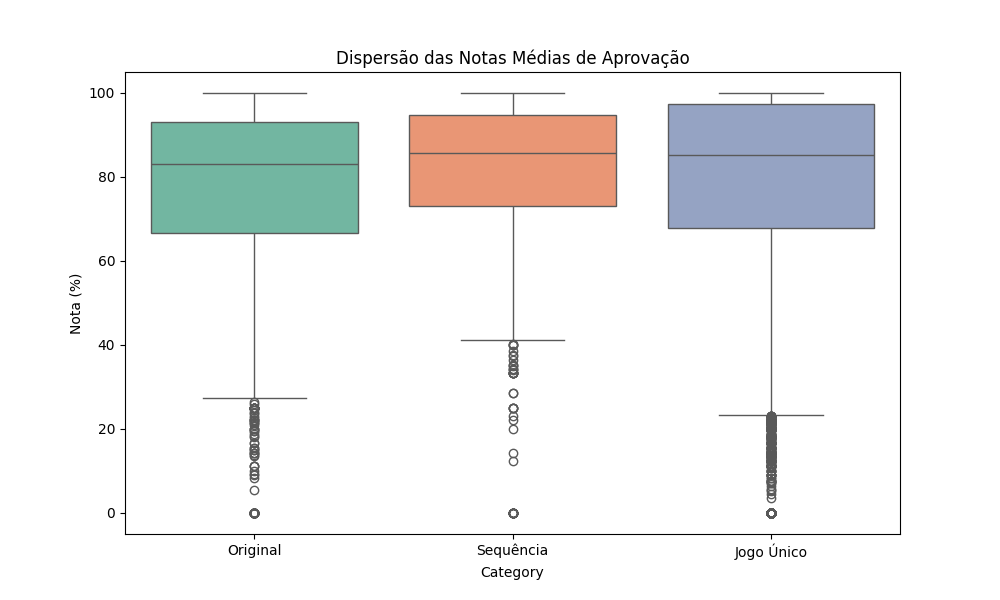
\includegraphics[width=\linewidth,height=0.38\textheight,keepaspectratio]{boxplot_scores.png}
            \end{center}
        \end{column}
    \end{columns}
\end{frame}
